\documentclass[10pt]{article}
% Submission version of the paper. The long working record (every run, development history) is docs/paper_draft.md;
% numbers here are taken from it and from docs/paper_assets (see CHECK.md). Figures: python docs/latex/figures.py.
\usepackage[letterpaper,textwidth=5.5in,textheight=9in,top=1in,headheight=12pt,headsep=25pt,footskip=30pt]{geometry}
\usepackage[T1]{fontenc}
\usepackage[utf8]{inputenc}
\usepackage{mathptmx}
\usepackage{microtype}
\usepackage{amsmath,amssymb,amsthm,mathtools}
\usepackage{booktabs,multirow,threeparttable}
\usepackage{graphicx}
\usepackage[font=small,labelfont=bf,skip=4pt]{caption}
\usepackage{enumitem}
\usepackage{xcolor}
\usepackage[numbers,sort&compress]{natbib}
\usepackage[hidelinks]{hyperref}
\usepackage[capitalise,nameinlink]{cleveref}

\setlist{nosep,leftmargin=*}
\renewcommand{\topfraction}{0.9}
\renewcommand{\bottomfraction}{0.6}
\renewcommand{\textfraction}{0.08}
\renewcommand{\floatpagefraction}{0.85}
\setcounter{topnumber}{3}
\setcounter{totalnumber}{4}

\setlength{\parskip}{0pt}
\theoremstyle{plain}
\newtheorem{theorem}{Theorem}
\newtheorem{lemma}[theorem]{Lemma}
\newtheorem{proposition}[theorem]{Proposition}
\newtheorem{corollary}[theorem]{Corollary}
\theoremstyle{definition}
\newtheorem{approximation}[theorem]{Approximation}
\crefname{approximation}{Approximation}{Approximations}

\newcommand{\E}{\mathbb{E}}
\newcommand{\R}{\mathbb{R}}
\newcommand{\LSE}{\mathrm{LSE}}
\newcommand{\KL}{\mathrm{KL}}
\newcommand{\ER}{\textsc{ER}}
\newcommand{\pos}[1]{\textbf{#1}}

\title{Where Does Heterogeneous Federated Learning Lose Rare Classes?\\
A Stage-by-Stage Comparison with Centralised Training}
\author{Anonymous authors\\Paper under double-blind review}
\date{}

\begin{document}
\maketitle

\begin{abstract}
Generator-based model-heterogeneous federated learning lets clients with different architectures share knowledge
through a frozen feature extractor, a conditional feature generator trained by federated averaging, and
architecture-specific heads. It has been evaluated only on balanced clients. We ask where, under long-tailed label
skew, such a pipeline loses accuracy relative to the \emph{same} pipeline trained on the pooled data. Since a client
partition is a pure label shift, federation cannot bias class-conditional targets; it loses accuracy only through the
optimiser, through parameters tied to a client's label prior, and through sample size. (i)~In the generator, Adam's
coupled weight decay on clients that lack a class shrinks that class's conditioning parameters at Adam's step size; a
ratio computed from class counts alone predicts the collapse (all 352 of 900 rows below threshold collapsed; 16 of 16
in a prospective test). (ii)~The largest loss, 7--20 points of balanced accuracy, is the last layer; a readout from
securely aggregated class statistics equals its centralised counterpart, whereas per-client logit corrections are
exact reparametrisations that cannot change the representation. (iii)~Synthetic features help the representation
only if they carry their label: label-independent synthetic data penalise the spread of the logits, and the gain of
the synthetic phase changes sign with the generator's signal fraction. Repairing each stage brings the pipeline within
0--2 points of centralised training where we could measure it, but on fresh seeds its margin over the strongest of
nine baselines is only $-0.3$ to $+1.9$ points. The collapse mechanism also removes rare item embeddings in federated
matrix factorisation.
\end{abstract}

% ---------------------------------------------------------------------------------------------------------------------
\section{Introduction}

Federated deployments rarely have one model architecture or balanced labels: sites run different networks on
different hardware, and rare classes are seen by few of them. Generator-based model-heterogeneous federated learning
(GeFL and its feature-space variant GeFL-F~\cite{kang2025gefl}) addresses the first problem. Parameters of different
architectures cannot be averaged, so the clients instead train a shared conditional generator by FedAvg~\cite{mcmahan2017},
and every architecture learns from its samples. Its evaluation used IID clients.

We study the second problem in this setting and ask a diagnostic question: \emph{when labels are long-tailed across
clients, how far is the federated solution from the centralised one, and which stage is responsible?} We compare each
stage of GeFL-F with its counterpart trained on the pooled data, with proofs where the question has an exact answer and
measurements where it does not. Our findings are:
\begin{enumerate}
\item \textbf{Federation adds no target bias} (\cref{sec:setting}): the partition is a pure label shift, and the
extractor is, to first order, trained on the pooled objective.
\item \textbf{The generator loses rare classes through the optimiser} (\cref{sec:generator}). With Adam and coupled
weight decay, a client that lacks a class moves that class's conditioning row toward zero at Adam's full step size,
while holders barely grow it. A count-only step ratio $\kappa_c$ predicts which rows collapse, retrospectively and
prospectively (\cref{fig:kappa}). Decoupled decay or averaging each row over its holders removes the collapse.
\item \textbf{The last layer is the largest loss and is recovered exactly} (\cref{sec:heads}). Per-client logit
corrections (logit adjustment, FedLC, FedRS, balanced softmax) are reparametrisations of a single-client head; a
readout from aggregated class statistics equals the centralised readout and recovers 7--20 points.
\item \textbf{Synthetic data help the representation only if they carry their label} (\cref{sec:signal}).
Label-independent synthetic data penalise the spread of the logits; the gain of the synthetic phase changes sign with
the generator's signal fraction (\cref{fig:signal}).
\end{enumerate}
We then repair each stage with exactly aggregated statistics (\cref{sec:method}) and test the result
(\cref{sec:experiments}). Where we could build the centralised comparator (MNIST, FashionMNIST, CIFAR-100), the
federated pipeline loses about as much to the long tail as centralised training does. Against nine baselines on fresh
seeds with validation-selected settings, however, its margin is small ($-0.3$ to $+1.9$ points): removing the coupled
decay and adding the exact readout recover most of the loss, which is itself a finding. Finally, the generator
mechanism is an instance of a general one: in federated matrix factorisation on MovieLens-1M, rare item embeddings
collapse in the same way (\cref{sec:recsys}).

\paragraph{Contributions.} (1)~A stage-by-stage decomposition of the federated--centralised gap, assembled from short
exact results (the tools are classical; the assembly is new), each checked against a measurement. (2)~A count-only
predictor of rare-class collapse in FedAvg-trained conditional models, confirmed retrospectively, prospectively and by
intervention. (3)~A measured ranking of the losses: last layer 7--20 points, generator collapse 7--11, one-client
representations 3--4, label-free synthetic data up to 2, extractor 0--1. (4)~A pre-registered evaluation with honest
margins, including the predictions that failed.

% ---------------------------------------------------------------------------------------------------------------------
\section{Setting and the centralised comparator}\label{sec:setting}

\paragraph{GeFL-F.} There are $K$ clients; client $k$ holds $D_k$ and trains a head of architecture $a(k)$ out of $G$
architectures. (1)~A small feature extractor (FE) $\phi$ is trained with the heads by FedAvg and frozen. (2)~A
conditional VAE $G_F(h\mid y)$ is trained on features $h=\phi(x)$ by FedAvg, with Adam (learning rate $10^{-3}$) and
\emph{coupled} weight decay $\lambda=10^{-3}$, as in~\cite{kang2025gefl}. The label enters through a linear projection
whose $c$-th column, the \emph{conditioning row} $r_c\in\R^d$, is the only class-specific parameter. (3)~Each round,
each client trains its head for $T_s$ epochs on generated features with uniformly drawn labels and then for $T_r=5$
epochs on its real features; heads of the same architecture are averaged.

\paragraph{Notation.} $n_{kc}$ is client $k$'s count of class $c$, $n_c=\sum_kn_{kc}$, $N=\sum_cn_c$,
$\pi_{kc}=n_{kc}/n_k$. $H_c$ is the set of $m_c$ clients holding $c$. A long-tailed split draws class sizes
$n_c\propto\mathrm{IF}^{-c/(C-1)}$, randomly permutes each class and cuts it into Dirichlet shares.

\begin{lemma}[pure label shift]\label{lem:labelshift}
For every client $k$ and class $c$ with $n_{kc}>0$, client $k$'s class-$c$ samples are a uniformly random subset of the
pooled class-$c$ samples. Hence $P_k(x\mid y)=P(x\mid y)$, and the same holds for $h=\phi(x)$.
\end{lemma}

So for any class-conditional quantity (a class row, a class mean, a readout) every client's data term points at the
centralised target. Federation can cost \emph{weighting, variance and rate}, but a \emph{bias} can only come from
(i)~the optimiser, (ii)~parameters coupled to a client's label prior (biases, last layers), or (iii)~shared parameters
trained on prior-weighted losses, which are equally prior-weighted centrally. \Cref{sec:generator,sec:heads} locate each.

\paragraph{The centralised comparator.} We compare against GeFL-F's own two-stage design trained on the pooled data:
an extractor (federated, or central with balanced sampling), then each architecture's body trained on the pooled real
features with the same schedule, then the same class-balanced readout. This isolates what federation costs given the
frozen-extractor design. The metric is balanced accuracy.

\paragraph{Stage I is first-order pooled training.} FedAvg with $p_k=1/K$ and $\tau_k\propto n_k$ local steps has, to
first order, the surrogate objective $\sum_k\frac{p_k\tau_k}{\bar\tau}\mathcal L_k$~\cite{wang2020fednova}, whose
weights on our splits equal $n_k/N$ up to a total variation of 0.009--0.018 at $K=10$ (\cref{app:proofs}). The regime
is not perturbative~\cite{charles2021,pathak2020}, so we test it directly: replacing the federated extractor by a centrally trained, class-balanced one changes the accuracy of a pooled
body with the exact readout by $0.0$, $+1.1$ and $-1.0$ points (MNIST, FashionMNIST, CIFAR-100; \cref{sec:central}).

% ---------------------------------------------------------------------------------------------------------------------
\section{Stage II: why the generator loses rare classes}\label{sec:generator}

\subsection{A contraction bound and the role of Adam}

In one round, client $k$ starts from the global row $r_c$, runs local Adam steps, and returns $r_{k,c}$. Let
$\Delta_k=\|r_{k,c}\|-\|r_c\|$, the holders' mean gain $\bar G_c=\frac1{m_c}\sum_{k\in H_c}\Delta_k$ and the
non-holders' mean loss $\bar D_c=-\frac1{K-m_c}\sum_{k\notin H_c}\Delta_k$; $p_c=m_c/K$.

\begin{theorem}[contraction bound]\label{thm:contraction}
Under flat averaging $r_c^+=\frac1K\sum_kr_{k,c}$,
\(\|r_c^+\|\le\|r_c\|+p_c\bar G_c-(1-p_c)\bar D_c\), with equality iff all $r_{k,c}$ are parallel. The row contracts
whenever $p_c<\theta_c:=\bar D_c/(\bar G_c+\bar D_c)$.
\end{theorem}

The bound is the triangle inequality applied to measured changes; it describes, it does not predict. What the optimiser
decides is the size of $\bar D_c$:

\begin{lemma}[coupled decay under Adam]\label{lem:adam}
A non-holder's gradient on $r_c$ is exactly $\lambda r_c$. Adam is invariant to a positive rescaling of the gradient
sequence up to $\epsilon$, so while $\lambda|r_{c,j}|\gg\epsilon$ each non-holder step moves every coordinate of $r_c$
toward zero by about the learning rate $\eta$, independently of $\lambda$. At $\lambda=0$, $\bar D_c=0$ exactly.
Under SGD the same decay costs only $\approx S\eta\lambda\|r_c\|$ per round.
\end{lemma}

A holder's data gradient fits the row and need not grow its norm, so $\bar G_c\ll\bar D_c$,
$\theta_c>\frac12$, and \emph{rare-class rows contract even when most clients hold the class}. On an instrumented run
(MNIST, IF $=100$, $K=10$) every class is held by at least 7 of 10 clients, yet the rows of the three rarest classes
shrank to 4--10\% of their initial norm while head rows grew by $1.4\times$. $\lambda=10^{-4}$ and $10^{-3}$ gave
the same trajectories (final tail/head ratio 0.155 vs 0.152); at $\lambda=0$ it stayed at 0.85. Since even a class held
by every client can contract when holder updates disagree in direction, no threshold on $m_c$ alone can be correct.

\subsection{A count-only predictor}

\begin{approximation}[step ratio]\label{app:kappa}
Per coordinate an Adam step is $\eta\psi$ with $\psi=\hat m/\sqrt{\hat v}\in[-1,1]$. A non-holder sees a constant-sign
decay gradient, so $\psi=\mathrm{sign}(r_{cj})$ on each of its $\tau_k$ steps; a holder moves the row only on its
$\tau_kf_{kc}$ steps whose batch contains $c$ ($f_{kc}$ is a hypergeometric probability), with $|\psi|\le1$. The drift
per round under flat averaging is therefore
\begin{equation}\label{eq:kappa}
\Delta r_{cj}=\tfrac{\eta}{K}\Big[\psi_h\!\sum_{k\in H_c}\!\tau_kf_{kc}-\mathrm{sign}(r_{cj})\!\sum_{k\notin H_c}\!\tau_k\Big],
\qquad \kappa_c=\frac{\sum_{k\in H_c}\tau_kf_{kc}}{\sum_{k\notin H_c}\tau_k}.
\end{equation}
If $\kappa_c<1$ the drift points toward zero for every coordinate and every target: the row collapses up to an
$O(\eta\tau/K)$ oscillation. If $\kappa_c>1$ it settles where the holders' normalised step is $1/\kappa_c$.
\end{approximation}
This neglects momentum carried between sparse holder steps and the drift of $\hat v$. $\kappa_c$ uses only the class
counts and the number of local steps, both known before training.

\begin{figure}[t]
\centering
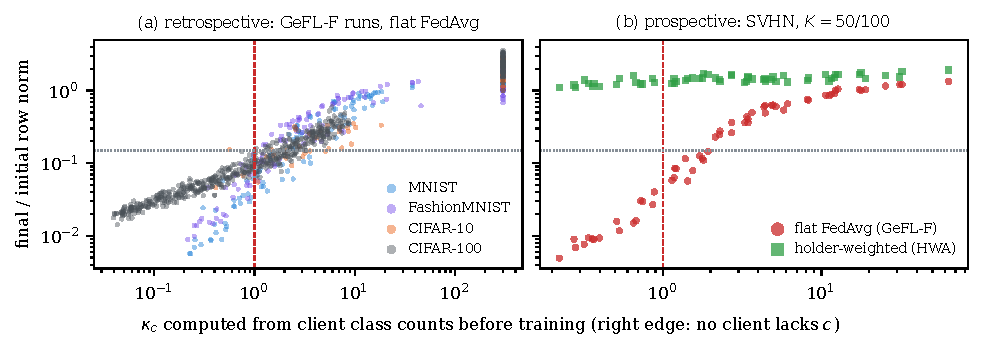
\includegraphics[width=0.95\linewidth]{fig_kappa.pdf}
\caption{Class counts alone predict the collapse of conditioning rows. Final over initial row norm against $\kappa_c$
(\cref{eq:kappa}); dashed: $\kappa_c=1$. (a)~All 900 logged rows of GeFL-F runs (MNIST, FashionMNIST at $K=10,50,100$;
CIFAR-10; CIFAR-100): all 352 rows with $\kappa_c<1$ end at $\le0.153$ of their initial norm; Spearman 0.94.
(b)~Prediction fixed before the runs: all 16 rows with $\kappa_c<1$ collapse under flat averaging (largest norm 0.04),
none under holder-weighted averaging (smallest 1.25).}
\label{fig:kappa}
\end{figure}

\Cref{fig:kappa}: $\kappa_c<1$ has been sufficient for collapse in all 368 rows; $\kappa_c\ge1$ is not sufficient to
survive when the holders' signal is weak. Instrumenting every round, the per-round shrinkage on non-holders is 2--10
times the holders' growth under coupled decay and about $10^{-3}$ or less with decoupled decay.

\paragraph{Why centralised Adam does not collapse these rows.} Centrally, $\hat v$ for $r_c$ is dominated by data
gradients, so decay steps are $\lambda r/\sqrt{\hat v}\ll\eta$, provided the row receives data more often than Adam's
second moment forgets ($1/(1-\beta_2)=1{,}000$ steps), as every class does here. In federation a non-holder's $\hat v$
contains only decay. When the frequency condition fails centrally too, as for rare items in recommendation,
centralised training collapses as well (\cref{sec:recsys}).

\subsection{Fixes: the optimiser or the aggregation}

If the coupled decay on non-holders causes the collapse, any fix that removes it should restore the rows.
\emph{Holder-weighted aggregation} (HWA) averages each row only over the clients that hold the class, with weights
$E(n_{kc})=(1-\beta^{n_{kc}})/(1-\beta)$~\cite{cui2019}, $\beta=0.999$:
$r_c\leftarrow\sum_kE(n_{kc})r_{k,c}/\sum_kE(n_{kc})$; it needs only two sums, so it runs under secure
aggregation~\cite{bonawitz2017}. It removes the $\bar D_c$ term of \cref{thm:contraction} and, without decay, also the
$m_c/K$ dilution of a rare row's learning rate (\cref{prop:dilution} in the appendix).

\begin{table}[t]
\centering\small
\caption{Fixing the collapse (balanced accuracy, long tail, 3 seeds, heads with LA). Every fix restores the rare rows
(tail/head norm 0.73--0.97 against 0.04--0.34).}
\label{tab:fixes}
\begin{tabular}{lcccccc}
\toprule
& \multicolumn{3}{c}{MNIST} & \multicolumn{3}{c}{FashionMNIST}\\
\cmidrule(lr){2-4}\cmidrule(lr){5-7}
$K$ & 10 & 50 & 100 & 10 & 50 & 100\\
\midrule
GeFL-F (coupled decay) & 79.2 & 81.4 & 79.5 & 65.2 & 66.5 & 66.6\\
+ AdamW (decoupled decay) & 86.4 & 84.7 & 81.6 & 75.9 & 74.0 & 71.8\\
+ no decay on class rows only & 86.8 & 84.4 & 81.8 & 75.9 & 74.5 & 71.9\\
+ HWA (coupled decay kept) & \pos{87.9} & \pos{86.5} & \pos{83.1} & 76.0 & \pos{75.5} & \pos{73.3}\\
\midrule
HWA $-$ best optimiser fix & $+1.1$ & $+1.8$ & $+1.3$ & $-0.1$ & $+0.9$ & $+1.4$\\
\bottomrule
\end{tabular}
\end{table}

\Cref{tab:fixes}: removing the coupled decay recovers 2--11 points; removing it only on the class rows is as good as
removing it globally, so the decay \emph{on the rows} is the cause. HWA adds 1.3--1.8 points at $K=50,100$ on MNIST,
the regime where the dilution of a rare row's rate is largest (the HWA/flat rate ratio of MNIST's rarest class is
1.15, 2.28 and 3.14 at $K=10,50,100$).

% ---------------------------------------------------------------------------------------------------------------------
\section{Stage III: heads, readout and synthetic data}\label{sec:heads}

\subsection{Per-client logit corrections are reparametrisations}

\begin{proposition}\label{prop:reparam}
Let a head have a free last-layer bias $b$, trained by SGD without decay on $b$, and let $a_k\in\R^C$ be a client
constant: logit adjustment $a_k=\tau\log\pi_k$~\cite{menon2021logit}, FedLC's calibration~\cite{zhang2022fedlc} or
balanced softmax. (1)~Training with $\ell(f+a_k,y)$ from $(\theta_0,b_0)$ produces exactly the trajectory of training
with $\ell(f,y)$ from $(\theta_0,b_0+a_k)$; every parameter except $b$ is identical at every step. (2)~FedRS~\cite{li2021fedrs},
which scales absent-class logits by $\alpha$, is plain cross-entropy in rescaled variables $\tilde w_c=\alpha w_c$,
$\tilde b_c=\alpha b_c$ with the learning rate on those rows multiplied by $\alpha^2$; the body follows the same trajectory.
\end{proposition}

For a single-client head trained on real data, these four published corrections therefore act only through the
readout. Measured on five datasets and three fresh seeds, real-data heads trained with cross-entropy, LA, FedLC or
FedRS reach the same exact-readout accuracy within 0.5 points on every seed and dataset. The identity breaks in two
places that matter here: when clients with different $a_k$ are averaged, and when a synthetic phase on unadjusted
logits alternates with an adjusted real phase (\cref{sec:signal}).

\subsection{The readout is partition-invariant}

\begin{theorem}[partition invariance]\label{thm:invariance}
Let an estimator be a function $\Psi(S)$ of $S=\sum_k\sum_{i\in D_k}T(x_i,y_i)$ with $T$ fixed in advance. Its value is
the same for every partition of the pooled data and equals the centralised estimator.
\end{theorem}

The theorem is trivial; its use is to sort the pipeline. The \emph{exact readout} (\ER) replaces each architecture's
last layer by the class-balanced linear discriminant computed from per-class counts, sums $\sum e$ and second moments
$\sum ee^\top$ of that architecture's embeddings $e$ over \emph{all} clients (one extra round): with class means $\mu_c$
and pooled within-class covariance $S$ shrunk to $S_\gamma=(1-\gamma)S+\gamma\frac{\mathrm{tr}S}{d}I$, $\gamma=0.1$,
it sets $w_c=S_\gamma^{-1}\mu_c$, $b_c=-\frac12\mu_c^\top S_\gamma^{-1}\mu_c$. By \cref{thm:invariance} \ER, Fed3R~\cite{fani2024fed3r},
FedNCM~\cite{legate2023fedncm} and all-client CCVR~\cite{luo2021ccvr} equal their centralised values for the same
bodies. The extractor, generator and bodies trained by FedAvg are not partition-invariant; neither are LA, FedLC and
FedRS, which are client-specific by design. Two consequences: the federated last layer stops being a source of loss
relative to centralised training of the same bodies; and \ER\ accuracy measures the body, not its last layer. A head
trained on one client is the extreme case of minority collapse~\cite{fang2021}: absent classes have imbalance ratio
$\infty$, and \ER\ sidesteps it.

\subsection{Alternation and the signal fraction}\label{sec:signal}

Each round a client runs $S_s$ synthetic steps, then $S_r$ real steps.
\begin{proposition}[alternation; quadratic losses]\label{prop:alternation}
Let the synthetic and real losses be quadratic with Hessians $H_s,H_r\succeq0$ and minimisers $\theta_s,\theta_r$;
$P_s=(I-\eta H_s)^{S_s}$, $P_r=(I-\eta H_r)^{S_r}$. If $\|P_rP_s\|<1$ the round map converges to
$\theta^\star=\theta_r+\Omega(\theta_s-\theta_r)$, $\Omega=(I-P_rP_s)^{-1}P_r(I-P_s)$. For commuting Hessians the
synthetic weight along eigendirection $i$ is $\omega_i=\rho_{r,i}(1-\rho_{s,i})/(1-\rho_{r,i}\rho_{s,i})\le\rho_{r,i}$.
\end{proposition}
Along directions the client's real loss leaves free ($h_{r,i}=0$) the synthetic data decide; these are exactly the
directions of the classes the client lacks. This gives logit adjustment a second role during training: without it the
real phase pushes absent-class logits down without bound, as on separable data~\cite{soudry2018}, and erases what the
synthetic phase taught. Measured on the real pipeline, the fraction of the synthetic phase's change to absent-class rows
that survives the next real phase is 0.96--1.0 with LA and 0.76--0.98 without.

What the synthetic phase teaches depends on whether its samples carry their label.
\begin{proposition}[label-free synthetic data penalise logit spread]\label{prop:variance}
If the synthetic label $y$ is uniform on $[C]$ and independent of the generated feature, then for every logit vector $f$
\[\E_y\,\ell(f,y)=\LSE(f)-\bar f=\log C+\KL\big(u\,\|\,\mathrm{softmax}f\big)=\log C+\tfrac1{2C}\textstyle\sum_c(f_c-\bar f)^2+O(\|f-\bar f\|^3).\]
If a generated sample carries its label's information with probability $s$ (the \emph{signal fraction}) and is
label-independent otherwise, the synthetic loss is $s\,\E[\ell\mid\text{faithful}]+(1-s)\,\E\,\KL(u\,\|\,p_f)$.
\end{proposition}

At $s\approx0$ the synthetic phase is an explicit anti-discrimination regulariser on the generator's support, and by
\cref{prop:alternation} it survives exactly in the absent-class directions. The prediction is a sign change: synthetic
data hurt the body when $s$ is near zero and help once the faithful term dominates. \Cref{fig:signal} confirms it. We
estimate $s=(a-1/C)/(1-1/C)$ from the accuracy $a$ of a referee classifier, trained on held-out real features, on
generated features. On CIFAR-100, GeFL-F's generator ($s=0.002$) makes the bodies $2.2$ points worse than training on
real data alone; the decay-fixed generator ($s=0.010$) $1.2$ points worse. Within every dataset the gain increases with
$s$. On the real pipeline, the spread of the logits on generated features after the synthetic phase relative to before
it settles at 0.5--0.6 for GeFL-F and 0.7--0.8 for the higher-$s$ generators, as \cref{prop:variance} predicts.

\begin{figure}[t]
\centering
\begin{minipage}[c]{0.46\linewidth}
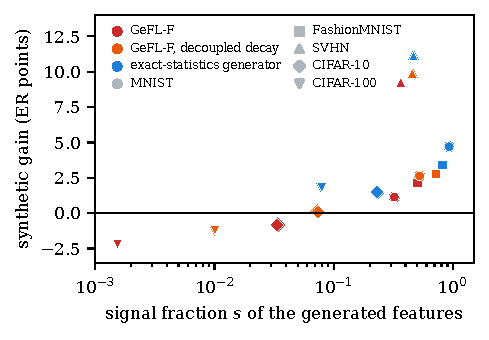
\includegraphics[width=\linewidth]{fig_signal.pdf}
\end{minipage}\hfill
\begin{minipage}[c]{0.5\linewidth}
\caption{The synthetic phase helps the representation only when generated features carry their label. Gain of the
synthetic phase (exact-readout accuracy minus that of heads trained on real data only, same seeds and splits) against
the signal fraction $s$ of the generated features; mean of three fresh seeds per point. The gain changes sign between
$s\approx0.03$ and $0.07$ (CIFAR-10, CIFAR-100). SVHN gains most at moderate $s$ because its real-only bodies are
the weakest.}
\label{fig:signal}
\end{minipage}
\end{figure}

% ---------------------------------------------------------------------------------------------------------------------
\section{Repairing each stage with exact statistics}\label{sec:method}

The diagnosis suggests one principle: wherever the data decide the result, use a statistic that secure aggregation
computes exactly (a sum over clients of per-class quantities) instead of a parameter that FedAvg estimates. Every
statistic below costs one upload per client and reveals only federation-level sums. The principle is not new as a
readout (CCVR, Fed3R, FedNCM); we apply it to the generator.

\paragraph{Generator.} (i)~\emph{Mean anchor.} The decoder models only the within-class residual,
$\tilde h=\mathrm{ReLU}(m_y+\mathrm{dec}(z,m_y))$, where $m_y$ is the exact class mean and enters through a
class-\emph{shared} projection. There is no class-specific parameter, so \cref{thm:contraction} has nothing to act on.
(ii)~\emph{Moment correction} (MC) rescales each class's samples to the exact class mean and spread; in idealised form
it is the minimum-displacement map with these moments (\cref{prop:mc}); after the final ReLU and with plug-in moments it
matches them only approximately. (iii)~\emph{Herding} (KH) selects, from $4\times$ candidates, the samples whose
random-Fourier-feature mean is closest to the exact class mean embedding. (iv)~\emph{Gate.} A mean anchor cannot separate
classes whose means are close (\cref{prop:w1}); the server computes the separation
$F=\overline{\|m_c-\bar m\|^2}/\overline{V_c}$ from the same sums and, if $F<0.05$, uses the original generator with
HWA instead. Measured $F$ is 0.005--0.013 on SVHN, 0.054--0.080 on CIFAR-10 and $\ge0.18$ elsewhere.

\paragraph{Heads and readout.} Heads use logit adjustment with the client's own prior and \emph{consensus soft labels}
(CSL) on synthetic features, $t(\tilde h)=\frac12e_y+\frac12\frac1G\sum_g\mathrm{softmax}\,h_g(\tilde h)$, the
averaged prediction of all architectures' heads on that feature~\cite{menon2021distillation}. After training, every
architecture's last layer is replaced by \ER. The \emph{minimal variant} for an existing deployment is the original
generator with HWA (or decoupled decay), LA, CSL and \ER.

% ---------------------------------------------------------------------------------------------------------------------
\section{Experiments}\label{sec:experiments}

\paragraph{Protocol.} We follow GeFL-F's published configuration~\cite{kang2025gefl}: a one-block frozen extractor, ten
CNN head architectures, CVAE-F, SGD for the heads. Datasets: MNIST, FashionMNIST, SVHN, CIFAR-10 and CIFAR-100-LT;
imbalance factor 100, Dirichlet(0.5) client shares, $K=10$ (one client per architecture) unless stated. On our
reproduction GeFL-F matches the published IID numbers within 0.5 points (MNIST 96.02 vs 95.47; FashionMNIST 82.67 vs
83.14). Metric: final-round balanced accuracy on balanced test sets. \emph{Development} results (seeds 0--2) chose
$T_s$, $\beta$, $\tau$ and the gate threshold on the test sets; the \emph{main comparison} (\cref{sec:fair}) uses fresh
seeds 3--5, chooses every method's readout and our $T_s$ on 2,000 held-out training images, fixed its selection rule
and predictions before any run, and reports paired 95\% CIs with Holm's correction. Details are in \cref{app:protocol}.

\subsection{Where the long-tail loss sits}

\begin{table}[t]
\centering\small\setlength{\tabcolsep}{4.5pt}
\caption{Every method under the same readout (development seeds 0--2, long tail). The exact readout lifts GeFL-F by
7--20 points; with the same readout, our bodies are 2.0--3.9 points better. Brackets: 95\% CI.}
\label{tab:readout}
\begin{tabular}{lccccc}
\toprule
& MNIST & FMNIST & SVHN & CIFAR-10 & CIFAR-100\\
\midrule
GeFL-F, heads as trained & 74.5 & 59.2 & 49.6 & 33.9 & 7.8\\
GeFL-F + \ER & 90.4 & 79.3 & 64.7 & 51.3 & 15.2\\
Minimal variant + \ER & 92.4 & 80.6 & 66.4 & 53.4 & 16.5\\
Ours, heads as trained & 95.1 & 80.1 & 65.4 & 45.7 & 15.4\\
Ours + \ER & \pos{94.4} & \pos{81.5} & \pos{66.7} & \pos{53.9} & \pos{18.6}\\
\midrule
Ours $-$ GeFL-F, both + \ER & $+3.9$ {\scriptsize[3.0, 4.8]} & $+2.2$ {\scriptsize[0.1, 4.4]} & $+2.0$ {\scriptsize[0.8, 3.2]} & $+2.6$ {\scriptsize[2.1, 3.1]} & $+3.4$ {\scriptsize[3.1, 3.8]}\\
\bottomrule
\end{tabular}
\end{table}

\Cref{tab:readout}: most of GeFL-F's long-tail loss is in the last layer ($+15.9$, $+20.1$, $+15.1$, $+17.4$, $+7.4$
points from \ER). Against a recalibrated GeFL-F, the gain of a better body is 2--4 points under every all-client
readout (CCVR $+2.1$ to $+3.6$; a pooled-real refit of the last layer $+2.6$ to $+4.5$). Published per-architecture
readouts use only an architecture's own clients and lose 4--26 points against their all-client versions.

\subsection{Fair re-test against nine baselines}\label{sec:fair}

\begin{table}[t]
\centering\small
\caption{Main comparison on fresh seeds 3--5, every method's readout (and our $T_s$) selected on validation data.
Ours minus baseline, test balanced accuracy, paired over seeds; brackets: 95\% CI; bold: Holm-adjusted $p<0.05$ over
nine baselines. The four real-data baselines with LA, FedLC, FedRS and balanced softmax coincide
(\cref{prop:reparam}); we show two.}
\label{tab:fair}
\setlength{\tabcolsep}{4pt}
\begin{tabular}{lccccc}
\toprule
& MNIST & FMNIST & SVHN & CIFAR-10 & CIFAR-100\\
\midrule
Ours (test accuracy) & 95.6 & 82.1 & 65.6 & 53.1 & 18.7\\
\midrule
$-$ GeFL-F & \pos{+3.4} {\scriptsize[3.2, 3.6]} & $+1.0$ {\scriptsize[$-$0.0, 2.1]} & $+1.5$ {\scriptsize[0.6, 2.5]} & \pos{+2.4} {\scriptsize[1.8, 3.0]} & \pos{+4.0} {\scriptsize[2.6, 5.4]}\\
$-$ GeFL-F, AdamW + LA & \pos{+2.0} {\scriptsize[1.9, 2.2]} & $+0.5$ {\scriptsize[$-$0.2, 1.2]} & $+1.5$ {\scriptsize[0.4, 2.6]} & $+1.5$ {\scriptsize[0.8, 2.2]} & \pos{+3.0} {\scriptsize[2.3, 3.7]}\\
$-$ real-data heads + LA & \pos{+4.7} & \pos{+2.6} & \pos{+11.3} & $+1.5$ & \pos{+1.6} {\scriptsize[0.7, 2.6]}\\
$-$ real-data heads + FedRS & \pos{+4.7} & \pos{+2.6} & \pos{+11.2} & $+1.6$ & \pos{+1.8}\\
$-$ Gaussian generator + LA & \pos{+2.9} {\scriptsize[1.7, 4.1]} & \pos{+1.3} {\scriptsize[1.3, 1.4]} & \pos{+12.4} & $+0.5$ {\scriptsize[$-$1.1, 2.1]} & \pos{+1.6} {\scriptsize[0.4, 2.8]}\\
$-$ FedDF & \pos{+1.9} {\scriptsize[1.4, 2.5]} & $+0.3$ {\scriptsize[$-$0.6, 1.2]} & $+0.5$ {\scriptsize[$-$1.0, 2.0]} & $+2.3$ {\scriptsize[0.9, 3.7]} & \pos{+3.5} {\scriptsize[2.5, 4.5]}\\
$-$ FedDF + LA & \pos{+2.0} {\scriptsize[1.2, 2.8]} & $+0.3$ {\scriptsize[$-$0.4, 1.0]} & $-0.3$ {\scriptsize[$-$1.6, 1.0]} & $+1.7$ {\scriptsize[0.4, 3.0]} & \pos{+3.5} {\scriptsize[2.2, 4.9]}\\
\midrule
margin over the strongest & \pos{+1.9} & $+0.3$ & $-0.3$ & $+0.5$ & \pos{+1.6}\\
\bottomrule
\end{tabular}
\end{table}

Baselines (\cref{tab:fair}): GeFL-F; GeFL-F with decoupled decay and LA; heads trained on real data only with LA,
FedLC, FedRS or balanced softmax; a Gaussian generator built from the same exact statistics, with LA (CCVR-style
virtual features during training); and server-side ensemble distillation (FedDF~\cite{lin2020feddf}) on generated
features, with and without LA. Each gets its own validation-selected readout. \textbf{Ours is not ahead of every
baseline:} the margin over the strongest is $-0.3$ to $+1.9$ points, significant on MNIST and CIFAR-100 only. Our
pre-registered prediction of at least 2 points over every baseline on four datasets \emph{failed}. FedDF is strong once
it gets an exact readout: distilling the ensemble into each head carries the ensemble's information even where the
generator's labels carry none. Removing the coupled decay and adding \ER\ recovers most of GeFL-F's loss; the
anchored generator adds 0.5--3.0 on top, and on CIFAR-100 it turns GeFL-F's harmful synthetic phase (14.8 vs 16.9 for
no synthetic data) into a gain ($+1.6$). Ablations are in \cref{app:ablation}.

\subsection{Federated versus centralised training}\label{sec:central}

\begin{table}[t]
\centering\small
\caption{Long-tail loss of the federated pipeline vs the centralised comparator (pooled real data, same
frozen-extractor design, same readout). CIFAR-100: three of the ten architectures; one seed.}
\label{tab:central}
\begin{tabular}{lccc}
\toprule
& MNIST & FashionMNIST & CIFAR-100\\
\midrule
Body trained on one client's real data + \ER & 91.5 & 78.1 & 15.1\\
Ours + \ER & 94.4 & 81.1 & 18.7\\
Pooled body + \ER, federated extractor & 94.4 & 81.9 & 18.1\\
\midrule
Long-tail drop, ours (balanced $\to$ long tail) & 2.9 & 3.3 & 2.7\\
Long-tail drop, centralised pipeline & 3.2 & 2.7 & 4.1\\
Federated residual (centralised $-$ ours) & 0.0 & 1.9 & $-0.6$\\
\bottomrule
\end{tabular}
\end{table}

\Cref{tab:central}: a body trained on one client loses 3.0--3.8 points against the pooled body; our synthetic data
recover all of it on MNIST and 80\% on FashionMNIST, and on CIFAR-100 our bodies reach the pooled level ($\pm1$). Our
federated pipeline loses about as much to the long tail as the centralised pipeline does: \emph{what remains is
largely the long tail itself, not federation.} FashionMNIST's 1.9-point residual is about 1.1 extractor and 0.8 body.
This also bounds what a better generator can still add over the decay-fixed baseline: if the pooled body is the ceiling, at most 1.9 points on
MNIST (we measure $+2.0$) and 1.4 on FashionMNIST (we measure $+0.5$). The small margins of \cref{tab:fair} are
therefore expected, not a failure of tuning. SVHN and CIFAR-10 were not measured.

\subsection{More clients and other imbalance settings}

\begin{table}[t]
\centering\small
\caption{Robustness (balanced accuracy with \ER; fresh seeds 3--5 unless stated). Left: several clients per
architecture. Right: ours minus the decay-fixed GeFL-F under other imbalance settings, FashionMNIST / SVHN.}
\label{tab:robust}
\setlength{\tabcolsep}{2.5pt}\footnotesize
\begin{tabular}{lccc}
\toprule
& \multicolumn{2}{c}{SVHN (seeds 0--2)} & CIFAR-10\\
$K$ & 50 & 100 & 50\\
\midrule
GeFL-F & 58.0 & 58.8 & --\\
AdamW + LA & 60.3 & 59.9 & 45.1\\
HWA + LA & 60.3 & 60.8 & 45.2\\
Ours & \pos{61.8} & \pos{61.0} & \pos{46.1}\\
\bottomrule
\end{tabular}\hfill
\begin{tabular}{lc}
\toprule
setting & ours $-$ decay fix\\
\midrule
IF $=10$ & $+1.0$ / $+2.6$\\
Dirichlet 0.1 & $+1.5$ / $+1.7$\\
Dirichlet 1.0 & $+0.8$ / $+1.0$\\
random rare classes & $+0.6$ / $+1.1$\\
\bottomrule
\end{tabular}
\end{table}

\Cref{tab:robust}. With several clients per architecture, HWA's advantage over decoupled decay is $+0.9$ with \ER\ on
SVHN at $K=100$ but about zero on CIFAR-10 at $K=50$ ($+0.1$, CI $[-0.2,0.4]$); ours is $+1.0$ ($[0.2,1.8]$), and every
method loses 6.5--7 points to $K=10$. Under other imbalance settings and with rare classes drawn at random, ours stays
ahead of both baselines in all eight cells, with a larger margin under stronger label skew (more absent classes leave
more room for synthetic data, \cref{prop:alternation}). The margins are small (three seeds).

\subsection{The same collapse in federated recommendation}\label{sec:recsys}

\Cref{sec:generator} needs only parameter rows used by few samples, clients that never use them, local Adam with
coupled L2, and plain averaging. Federated matrix factorisation has all four~\cite{chai2021fedmf}: item embeddings are shared and averaged, user embeddings stay local. On
MovieLens-1M~\cite{harper2015} (explicit ratings, users assigned at random to $K=10$ or $50$ clients, $d=32$, 30 rounds,
three seeds; predictions fixed before the runs), $\kappa_c<1$ for 895 of 3,706 items at $K=10$ and 2,108 at $K=50$.

\begin{table}[t]
\centering\small
\caption{Rare-item collapse in federated matrix factorisation (MovieLens-1M). Items with $\kappa_c<1$; collapsed:
final norm $\le0.15$ of initial.}
\label{tab:recsys}
\begin{tabular}{lccc}
\toprule
& collapsed & RMSE on these items & RMSE overall\\
& $K=10$ / $50$ & $K=10$ / $50$ & $K=10$ / $50$\\
\midrule
Adam + coupled L2, FedAvg & 85.0\% / 83.4\% & 1.094 / 1.064 & 0.859 / 0.908\\
AdamW, FedAvg & 0\% / 0\% & 1.036 / 0.992 & 0.904 / 0.907\\
Adam + L2, HWA & 23.3\% / 8.7\% & 1.042 / \pos{0.967} & \pos{0.857} / \pos{0.894}\\
SGD + L2, FedAvg & 0\% / 0\% & 1.160 / 1.144 & 0.967 / 1.010\\
centralised Adam + coupled L2 & 78.0\% & 1.099 & 0.888\\
\bottomrule
\end{tabular}
\end{table}

\Cref{tab:recsys}: $\kappa_c$ ranks the collapse (Spearman with the final norm 0.93 / 0.96), the collapsed share of
all items grows with $K$ (22\% to 48\%), and it costs accuracy on these items. Two of our four predictions failed: not
every $\kappa_c<1$ item collapses (83--85\% do), and \emph{centralised} Adam with coupled L2 collapses 78\% of them,
because they receive data less often than once per 1,000 steps (\cref{sec:generator}). The share of optimiser steps
whose batch contains the item predicts the final norm in both regimes (Spearman 0.91 central, 0.94--0.97 federated),
and at $K=50$ federation collapses moderately rare items about ten times harder. In recommendation, federation adds
severity rather than the existence of collapse. Count-weighted item aggregation is known~\cite{perifanis2022fedncf} and degraded item embeddings in federated
recommendation have been reported~\cite{shen2025embedding}; we are not aware of an account of the optimiser mechanism
or of a count-based predictor.

\paragraph{What did not work.} A server-side signal-fraction gate, a class-balanced extractor loss and recomputing
the exact readout during training did not help our method (\cref{app:negative}).

% ---------------------------------------------------------------------------------------------------------------------
\section{Related work}

\paragraph{Model-heterogeneous FL.} Methods exchange predictions on public or generated data
(FedMD~\cite{li2019fedmd}, FedDF~\cite{lin2020feddf}, FedGKT~\cite{he2020fedgkt}), keep part of the network local
(LG-FedAvg~\cite{liang2019lg}, FedRep~\cite{collins2021fedrep}, FedProto~\cite{tan2022fedproto}), train a server-side
generator against the client ensemble (FedGen~\cite{zhu2021fedgen}, FedFTG~\cite{zhang2022fedftg},
DENSE~\cite{zhang2022dense}), share statistics (FedVTC~\cite{niu2026fedvtc}, Felo/Velo~\cite{chan2025}), or train the
generator itself by FedAvg (GeFL~\cite{kang2025gefl}). FedGen and FedFTG weight teacher \emph{losses} by label counts;
HWA weights the \emph{parameters} of a client-trained generator, and our contribution is the mechanism behind it.

\paragraph{Federated learning under label skew and long tails.} Classifier re-calibration from federated statistics
(CCVR~\cite{luo2021ccvr}, CReFF~\cite{shang2022creff}, Fed3R~\cite{fani2024fed3r}, FedNCM~\cite{legate2023fedncm}) and
loss corrections by client label frequencies (FedLC~\cite{zhang2022fedlc}, FedRS~\cite{li2021fedrs},
FedRoD~\cite{chen2022fedrod}, BalanceFL~\cite{shuai2022balancefl}, Fed-GraB~\cite{xiao2023fedgrab},
FedLoGe~\cite{xiao2024fedloge}) are established. \Cref{prop:reparam} explains why the loss corrections coincide for a
single-client head, and \cref{thm:invariance} why the all-client readouts recover the last layer exactly. Class
embeddings can collapse under FedAvg when clients see only positive labels~\cite{yu2020fedaws}, a different cause.

\paragraph{Long tails, optimisers and synthetic data.} We build on logit adjustment~\cite{menon2021logit}, effective
numbers~\cite{cui2019} and decoupled classifiers~\cite{kang2020decoupling}; the collapse rests on coupled versus
decoupled decay in Adam~\cite{loshchilov2019,kingma2015}. Conditional generators can collapse on limited classes
centrally~\cite{shahbazi2022}, and synthetic training data are limited by label fidelity~\cite{ravuri2019cas}.

% ---------------------------------------------------------------------------------------------------------------------
\section{Limitations and conclusion}

\paragraph{Limitations.} Our margins over strong baselines are small; the claim is the decomposition, not a new
state of the art. The extractor is small and frozen, as in GeFL-F. The centralised comparison covers three datasets
with one seed, and only the fresh-seed comparison chose settings without test data. The theory uses models, so we draw
only ranking and sign claims from it, each paired with a measurement. The released class sums leak membership for rare
classes unless noised (\cref{app:privacy}). The recommendation result rests on one dataset.

\paragraph{Conclusion.} Heterogeneous FL loses rare classes in three places: the optimiser's treatment of clients
that lack a class, a last layer fitted to one client's prior, and synthetic data without label information. Each has an
exact description and a direct fix; what remains is largely the cost of the long tail itself.

% ---------------------------------------------------------------------------------------------------------------------
\small
\bibliographystyle{plainnat}
\begin{thebibliography}{99}
\bibitem[Kang et~al.(2025)]{kang2025gefl} H.~Kang, S.~Cha, and J.~Kang. GeFL: Model-agnostic federated learning with generative models. \emph{IEEE Transactions on Mobile Computing}, 2025. arXiv:2412.18460.
\bibitem[McMahan et~al.(2017)]{mcmahan2017} H.~B. McMahan, E.~Moore, D.~Ramage, S.~Hampson, and B.~Ag\"uera y~Arcas. Communication-efficient learning of deep networks from decentralized data. In \emph{AISTATS}, 2017.
\bibitem[Li and Wang(2019)]{li2019fedmd} D.~Li and J.~Wang. FedMD: Heterogenous federated learning via model distillation. NeurIPS Workshop on Federated Learning, 2019.
\bibitem[Lin et~al.(2020)]{lin2020feddf} T.~Lin, L.~Kong, S.~U. Stich, and M.~Jaggi. Ensemble distillation for robust model fusion in federated learning. In \emph{NeurIPS}, 2020.
\bibitem[He et~al.(2020)]{he2020fedgkt} C.~He, M.~Annavaram, and S.~Avestimehr. Group knowledge transfer: Federated learning of large CNNs at the edge. In \emph{NeurIPS}, 2020.
\bibitem[Liang et~al.(2019)]{liang2019lg} P.~P. Liang, T.~Liu, L.~Ziyin, N.~B. Allen, R.~P. Auerbach, D.~Brent, R.~Salakhutdinov, and L.-P. Morency. Think locally, act globally: Federated learning with local and global representations. NeurIPS Workshop on Federated Learning, 2019.
\bibitem[Collins et~al.(2021)]{collins2021fedrep} L.~Collins, H.~Hassani, A.~Mokhtari, and S.~Shakkottai. Exploiting shared representations for personalized federated learning. In \emph{ICML}, 2021.
\bibitem[Tan et~al.(2022)]{tan2022fedproto} Y.~Tan, G.~Long, L.~Liu, T.~Zhou, Q.~Lu, J.~Jiang, and C.~Zhang. FedProto: Federated prototype learning across heterogeneous clients. In \emph{AAAI}, 2022.
\bibitem[Zhu et~al.(2021)]{zhu2021fedgen} Z.~Zhu, J.~Hong, and J.~Zhou. Data-free knowledge distillation for heterogeneous federated learning. In \emph{ICML}, 2021.
\bibitem[Zhang et~al.(2022a)]{zhang2022fedftg} L.~Zhang, L.~Shen, L.~Ding, D.~Tao, and L.-Y. Duan. Fine-tuning global model via data-free knowledge distillation for non-IID federated learning. In \emph{CVPR}, 2022.
\bibitem[Zhang et~al.(2022b)]{zhang2022dense} J.~Zhang, C.~Chen, B.~Li, L.~Lyu, S.~Wu, S.~Ding, C.~Shen, and C.~Wu. DENSE: Data-free one-shot federated learning. In \emph{NeurIPS}, 2022.
\bibitem[Chan and Ngai(2025)]{chan2025} Y.-H. Chan and E.~C.-H. Ngai. Exploiting features and logits in heterogeneous federated learning. \emph{Computer Networks}, 2025.
\bibitem[Niu et~al.(2026)]{niu2026fedvtc} Z.~Niu, H.~Dong, and A.~K. Qin. Bridging generalization gap of heterogeneous federated clients using generative models. In \emph{ICLR}, 2026.
\bibitem[Luo et~al.(2021)]{luo2021ccvr} M.~Luo, F.~Chen, D.~Hu, Y.~Zhang, J.~Liang, and J.~Feng. No fear of heterogeneity: Classifier calibration for federated learning with non-IID data. In \emph{NeurIPS}, 2021.
\bibitem[Shang et~al.(2022)]{shang2022creff} X.~Shang, Y.~Lu, G.~Huang, and H.~Wang. Federated learning on heterogeneous and long-tailed data via classifier re-training with federated features. In \emph{IJCAI}, 2022.
\bibitem[Zhang et~al.(2022c)]{zhang2022fedlc} J.~Zhang, Z.~Li, B.~Li, J.~Xu, S.~Wu, S.~Ding, and C.~Wu. Federated learning with label distribution skew via logits calibration. In \emph{ICML}, 2022.
\bibitem[Li and Zhan(2021)]{li2021fedrs} X.-C. Li and D.-C. Zhan. FedRS: Federated learning with restricted softmax for label distribution non-IID data. In \emph{KDD}, 2021.
\bibitem[Shuai et~al.(2022)]{shuai2022balancefl} X.~Shuai, Y.~Shen, S.~Jiang, Z.~Zhao, Z.~Yan, and G.~Xing. BalanceFL: Addressing class imbalance in long-tail federated learning. In \emph{IPSN}, 2022.
\bibitem[Xiao et~al.(2023)]{xiao2023fedgrab} Z.~Xiao, Z.~Chen, S.~Liu, H.~Wang, Y.~Feng, J.~Hao, J.~T. Zhou, J.~Wu, H.~H. Yang, and Z.~Liu. Fed-GraB: Federated long-tailed learning with self-adjusting gradient balancer. In \emph{NeurIPS}, 2023.
\bibitem[Xiao et~al.(2024)]{xiao2024fedloge} Z.~Xiao, Z.~Chen, et~al. FedLoGe: Joint local and generic federated learning under long-tailed data. In \emph{ICLR}, 2024.
\bibitem[Chen and Chao(2022)]{chen2022fedrod} H.-Y. Chen and W.-L. Chao. On bridging generic and personalized federated learning for image classification. In \emph{ICLR}, 2022.
\bibitem[Fan{\`\i} et~al.(2024)]{fani2024fed3r} E.~Fan{\`\i}, R.~Camoriano, B.~Caputo, and M.~Ciccone. Accelerating heterogeneous federated learning with closed-form classifiers. In \emph{ICML}, 2024.
\bibitem[Legate et~al.(2023)]{legate2023fedncm} G.~Legate, N.~Bernier, L.~Page-Caccia, E.~Oyallon, and E.~Belilovsky. Guiding the last layer in federated learning with pre-trained models. In \emph{NeurIPS}, 2023.
\bibitem[Yu et~al.(2020)]{yu2020fedaws} F.~X. Yu, A.~S. Rawat, A.~K. Menon, and S.~Kumar. Federated learning with only positive labels. In \emph{ICML}, 2020.
\bibitem[Cui et~al.(2019)]{cui2019} Y.~Cui, M.~Jia, T.-Y. Lin, Y.~Song, and S.~Belongie. Class-balanced loss based on effective number of samples. In \emph{CVPR}, 2019.
\bibitem[Menon et~al.(2021a)]{menon2021logit} A.~K. Menon, S.~Jayasumana, A.~S. Rawat, H.~Jain, A.~Veit, and S.~Kumar. Long-tail learning via logit adjustment. In \emph{ICLR}, 2021.
\bibitem[Menon et~al.(2021b)]{menon2021distillation} A.~K. Menon, A.~S. Rawat, S.~Reddi, S.~Kim, and S.~Kumar. A statistical perspective on distillation. In \emph{ICML}, 2021.
\bibitem[Kang et~al.(2020)]{kang2020decoupling} B.~Kang, S.~Xie, M.~Rohrbach, Z.~Yan, A.~Gordo, J.~Feng, and Y.~Kalantidis. Decoupling representation and classifier for long-tailed recognition. In \emph{ICLR}, 2020.
\bibitem[Loshchilov and Hutter(2019)]{loshchilov2019} I.~Loshchilov and F.~Hutter. Decoupled weight decay regularization. In \emph{ICLR}, 2019.
\bibitem[Kingma and Ba(2015)]{kingma2015} D.~P. Kingma and J.~Ba. Adam: A method for stochastic optimization. In \emph{ICLR}, 2015.
\bibitem[Shahbazi et~al.(2022)]{shahbazi2022} M.~Shahbazi, M.~Danelljan, D.~P. Paudel, and L.~Van~Gool. Collapse by conditioning: Training class-conditional GANs with limited data. In \emph{ICLR}, 2022.
\bibitem[Ravuri and Vinyals(2019)]{ravuri2019cas} S.~Ravuri and O.~Vinyals. Classification accuracy score for conditional generative models. In \emph{NeurIPS}, 2019.
\bibitem[Fang et~al.(2021)]{fang2021} C.~Fang, H.~He, Q.~Long, and W.~J. Su. Exploring deep neural networks via layer-peeled model: Minority collapse in imbalanced training. \emph{PNAS}, 118(43), 2021.
\bibitem[Soudry et~al.(2018)]{soudry2018} D.~Soudry, E.~Hoffer, M.~S. Nacson, S.~Gunasekar, and N.~Srebro. The implicit bias of gradient descent on separable data. \emph{JMLR}, 19(70):1--57, 2018.
\bibitem[Wang et~al.(2020)]{wang2020fednova} J.~Wang, Q.~Liu, H.~Liang, G.~Joshi, and H.~V. Poor. Tackling the objective inconsistency problem in heterogeneous federated optimization. In \emph{NeurIPS}, 2020.
\bibitem[Charles and Kone{\v{c}}n{\'y}(2021)]{charles2021} Z.~Charles and J.~Kone{\v{c}}n{\'y}. Convergence and accuracy trade-offs in federated learning and meta-learning. In \emph{AISTATS}, 2021.
\bibitem[Pathak and Wainwright(2020)]{pathak2020} R.~Pathak and M.~J. Wainwright. FedSplit: An algorithmic framework for fast federated optimization. In \emph{NeurIPS}, 2020.
\bibitem[Bonawitz et~al.(2017)]{bonawitz2017} K.~Bonawitz, V.~Ivanov, B.~Kreuter, A.~Marcedone, H.~B. McMahan, S.~Patel, D.~Ramage, A.~Segal, and K.~Seth. Practical secure aggregation for privacy-preserving machine learning. In \emph{ACM CCS}, 2017.
\bibitem[Chai et~al.(2021)]{chai2021fedmf} D.~Chai, L.~Wang, K.~Chen, and Q.~Yang. Secure federated matrix factorization. \emph{IEEE Intelligent Systems}, 36(5):11--20, 2021.
\bibitem[Harper and Konstan(2015)]{harper2015} F.~M. Harper and J.~A. Konstan. The MovieLens datasets: History and context. \emph{ACM Transactions on Interactive Intelligent Systems}, 5(4), 2015.
\bibitem[Perifanis and Efraimidis(2022)]{perifanis2022fedncf} V.~Perifanis and P.~S. Efraimidis. Federated neural collaborative filtering. \emph{Knowledge-Based Systems}, 242, 2022.
\bibitem[Shen et~al.(2025)]{shen2025embedding} J.~Shen, Y.~Mi, G.~Zhao, J.~Shen, and X.~Qian. A model-agnostic strategy to mitigate embedding degradation in personalized federated recommendation. arXiv:2508.19591, 2025.
\bibitem[Gelbrich(1990)]{gelbrich1990} M.~Gelbrich. On a formula for the L2 Wasserstein metric between measures on Euclidean and Hilbert spaces. \emph{Mathematische Nachrichten}, 147:185--203, 1990.
\end{thebibliography}
\normalsize

% ---------------------------------------------------------------------------------------------------------------------
\clearpage
\appendix
\section{Proofs}\label{app:proofs}

\paragraph{\Cref{lem:labelshift}.} Given the counts, each contiguous chunk of a uniformly random permutation of a
class's indices is a uniformly random subset; the step that guarantees a minimum client size moves uniformly random
samples and preserves exchangeability within a class. Since $\phi$ is shared, $h=\phi(x)$ inherits the property.
\hfill$\square$

\paragraph{Stage I.} The one-round expansion of local SGD gives the aggregate update
$-\eta\bar\tau\nabla\tilde{\mathcal L}+O(\eta^2LG\tau^2)$ with $\tilde{\mathcal L}=\sum_k\frac{p_k\tau_k}{\bar\tau}\mathcal L_k$
\cite{wang2020fednova}. With $p_k=1/K$ and $\tau_k=\lfloor 5n_k/B\rfloor$ (batches of size one skipped) the weights are
$n_k/N$ up to the rounding, whose total variation we computed on every split used. \hfill$\square$

\paragraph{\Cref{thm:contraction}.} $\|\frac1K\sum_kr_{k,c}\|\le\frac1K\sum_k\|r_{k,c}\|=\|r_c\|+\frac1K\big(\sum_{k\in
H_c}\Delta_k+\sum_{k\notin H_c}\Delta_k\big)$; the two sums are $m_c\bar G_c$ and $-(K-m_c)\bar D_c$. Equality in the
triangle inequality holds iff all vectors are non-negative multiples of one another. \hfill$\square$

\paragraph{\Cref{lem:adam}.} A non-holder's batches contain no sample of class $c$, so the data loss does not depend on
$r_c$ and the coupled-decay gradient is $\lambda r_c$. Adam's update $\eta\hat m/(\sqrt{\hat v}+\epsilon)$ is unchanged
when the whole gradient sequence is multiplied by $a>0$, up to the $\epsilon$ term; hence the step does not depend on
$\lambda$ while $\lambda|r_{c,j}|\gg\epsilon$. Numerically the invariance holds for $\lambda\gtrsim10^{-5}$ at the
measured row norms. Each client keeps its Adam state across rounds while its parameters are reset to the global ones,
so a single step can exceed $\eta$. \hfill$\square$

\paragraph{\Cref{prop:reparam}.} (1) $f+a_k=Wu(h)+(b+a_k)$, and $b\mapsto b+a_k$ is a translation with identity
Jacobian, so gradients agree at corresponding points; induct over steps. (2) $\alpha f_c=\tilde w_c^\top u+\tilde b_c$;
the gradient in $\tilde w_c$ is $1/\alpha$ times that in $w_c$, so a step of size $\eta$ on $w_c$ is a step of
$\eta\alpha^2$ on $\tilde w_c$, and the body sees the same logits. Numerically the identity holds to $4\times10^{-16}$.
\hfill$\square$

\paragraph{\Cref{thm:invariance}.} Addition is associative and commutative. In particular every exponential-family
maximum-likelihood estimate, and the class-balanced LDA of \ER, is computed exactly by one round of secure aggregation.
\hfill$\square$

\paragraph{\Cref{prop:alternation}.} One round is the affine map $\theta\mapsto P_rP_s\theta+P_r(I-P_s)\theta_s+(I-P_r)\theta_r$.
If $\|P_rP_s\|<1$ it is a contraction with fixed point $\theta^\star=(I-P_rP_s)^{-1}[P_r(I-P_s)\theta_s+(I-P_r)\theta_r]$;
writing $(I-P_r)=(I-P_rP_s)-P_r(I-P_s)$ gives the stated form. With commuting Hessians all matrices are diagonal in a
common eigenbasis. \hfill$\square$

\paragraph{\Cref{prop:variance}.} $\frac1C\sum_c(\LSE(f)-f_c)=\LSE(f)-\bar f$ and $\KL(u\|\mathrm{softmax}f)=-\log
C+\LSE(f)-\bar f$; expanding $\LSE$ around constant logits gives the quadratic term. The mixture form follows by
conditioning on whether a sample is faithful. \hfill$\square$

\begin{proposition}[dilution without decay; quadratic row model]\label{prop:dilution}
Let client $k$'s class-$c$ loss be quadratic, $\frac12\sum_{i\in D_{kc}}\|r-t_i\|_A^2$. A local round then maps
$r$ to $M_{kc}r+(I-M_{kc})\bar t_{kc}$, and flat FedAvg converges to
\[r^*=\Big(\sum\nolimits_{H_c}(I-M_{kc})\Big)^{-1}\sum\nolimits_{H_c}(I-M_{kc})\bar t_{kc}\]
at a rate diluted by $m_c/K$. With saturated local training ($M_{kc}\to0$) its mean squared error is
$V_c=\frac{n_c}{m_c^2}\sum_{k\in H_c}1/n_{kc}\ge1$ times that of the pooled estimate, with equality iff all holders
have equal counts; HWA with weights $E(n_{kc})$ gives $V_c\approx1$.
\end{proposition}
\emph{Proof.} Non-holders contribute the identity map and drop out of the fixed-point equation; the rest is the
fixed-point formula for quadratic clients and the variance of independent unbiased local means (\cref{lem:labelshift}).
On the actual MNIST counts simulated error ratios match $V_c$ to two decimals. \hfill$\square$

\begin{proposition}[what a mean anchor can express]\label{prop:w1}
Let the class-$c$ sampler be $X_c=\mathrm{ReLU}(m_c+g(Z,Am_c))$ with $Z$ shared across classes and $g$ $L$-Lipschitz
in its second argument. Then $W_1(G_c,G_{c'})\le(1+L\|A\|_2)\|m_c-m_{c'}\|$.
\end{proposition}
\emph{Proof.} Couple both classes through the same $Z$; ReLU is 1-Lipschitz. \hfill$\square$

In units of the within-class spread, the anchors are on average $\sqrt{2F}$ apart. On SVHN ($F\approx0.005$--$0.013$)
they differ by 10--15\% of the spread, which is why the gate of \cref{sec:method} falls back to class rows there.

\begin{proposition}[minimum-displacement moment correction]\label{prop:mc}
Among all maps $T$ with $\E\,T(X)=m_c$ and $\E\|T(X)-m_c\|^2=V_c$, where $X$ has mean $\tilde m_c$ and spread $\tilde V_c$,
the map $T^\star(x)=m_c+\sqrt{V_c/\tilde V_c}\,(x-\tilde m_c)$ minimises $\E\|T(X)-X\|^2$. With exact covariances
instead of spreads the minimiser is the linear map attaining the Gelbrich bound~\cite{gelbrich1990}.
\end{proposition}
\emph{Proof.} With $Y=T(X)$, $\E\|Y-X\|^2=V_c+\tilde V_c+\|m_c-\tilde m_c\|^2-2\E\langle Y-m_c,X-\tilde m_c\rangle$, and
Cauchy--Schwarz bounds the last expectation by $\sqrt{V_c\tilde V_c}$, with equality iff $Y-m_c=\sqrt{V_c/\tilde
V_c}(X-\tilde m_c)$. \hfill$\square$

The deployed map applies a final ReLU and uses moments estimated from a finite batch, so it matches the moments only
approximately.

\section{Experimental details}\label{app:protocol}

\paragraph{Models and optimisation.} Extractor, heads (CNN-1 to CNN-10) and CVAE-F as in GeFL-F's appendix; CIFAR
extractors have ten output channels. Heads: SGD, learning rate 0.1. Rounds for extractor / generator / heads 20/100/50
on MNIST and FashionMNIST, and as published elsewhere. Data fraction 0.1 (0.5 for CIFAR-10, 0.22 for CIFAR-100, which
gives the standard CIFAR-100-LT shape: 480 images in the largest class and 5 in the smallest). Client-to-architecture
assignment is contiguous. With IF $=100$ the rarest classes are held by 6--8 of 10 clients; CIFAR-10's realised
imbalance is 48:1 because the rarest classes are capped by the data fraction.

\paragraph{Selection and statistics.} Fresh-seed runs choose every method's readout among heads as trained, balanced
bias calibration, \ER, Fed3R, FedNCM and CCVR (all-client or own-client) by validation balanced accuracy, and our
$T_s\in\{1,10\}$ the same way. Each seed fixes the split and the initialisations for every method; GPU training is not
bit-deterministic (a repeated seed differs by $-0.06\pm0.43$ points with \ER\ over 21 paired runs). CIs are paired
$t$-intervals over seeds.

\paragraph{The balanced setting.} With IID clients ours is within $+0.1$ to $+1.6$ points of GeFL-F with \ER\ (MNIST
97.4 vs 96.9, FashionMNIST 84.8 vs 84.5, CIFAR-10 61.6 vs 61.4, SVHN 77.3 vs 76.2, CIFAR-100 21.4 vs 19.8); the gain is
significant on SVHN and CIFAR-100 only. Holder-weighted averaging equals FedAvg when all clients have equal counts.

\section{Ablation and mechanism controls}\label{app:ablation}

Five seeds, heads as trained: removing any component lowers MNIST accuracy in every seed (LA $-3.05$, mean anchor
$-3.89$, CSL $-1.35$, MC $-1.13$, KH $-0.67$); on FashionMNIST LA $-5.78$, CSL $-1.50$, KH $-0.65$ (5 of 5), MC $-0.63$
and mean anchor $-0.50$ (4 of 5). With \ER: LA $+0.11$ / $+0.05$ (its contribution vanishes, as \cref{prop:reparam}
requires), CSL $-0.44$ / $-0.53$, MC $-0.53$ / $-0.14$, KH $-0.26$ / $-0.13$ (MNIST / FashionMNIST). Controls with one
shared generator per seed: herding beats a random subset of the same candidates (small but consistent); MC's gain comes
from the spread, not the mean (mean-only correction loses 0.9--1.0 points although it raises the referee's tail
fidelity by 4--5 points); results are flat in the random-feature dimension and the candidate-pool size.

\section{Privacy and cost}\label{app:privacy}

\begin{table}[h]
\centering\small
\caption{Membership inference on the released class sums (AUC; all classes / tail classes / rarest class).}
\begin{tabular}{lcc}
\toprule
release & MNIST & FashionMNIST\\
\midrule
exact sums & 0.52 / 0.64 / 0.69 & 0.52 / 0.63 / 0.73\\
Gaussian mechanism, $\varepsilon=8$ & 0.50 / 0.58 / 0.64 & 0.52 / 0.54 / 0.45\\
Gaussian mechanism, $\varepsilon=2$ & 0.50 / 0.53 / 0.61 & 0.51 / 0.50 / 0.41\\
\bottomrule
\end{tabular}
\end{table}

An attacker who knows a target's label and holds public reference data scores it by how far the released class mean
moved toward it. Head classes are at chance; the exact release leaks membership for rare classes (24--112 samples), as
expected for a mean over few samples. Formal differential privacy on the four statistics our generator adds costs
4.5--6.9 points at $\varepsilon=8$ and 9.8--14.1 at $\varepsilon=2$, still above GeFL-F at $\varepsilon=2$ on MNIST and
FashionMNIST; it does not cover the generator's FedAvg training or the heads. Our pipeline is 2.2--2.8$\times$ slower
than GeFL-F end to end (herding dominates the head stage); \ER\ adds one round and up to about $5\times10^5$ numbers per
architecture per client.

\section{Further negative results}\label{app:negative}

A server-side estimate of the signal fraction used as a gate helps the decay-fixed GeFL-F on the CIFARs ($+0.8$,
$+1.3$) but not ours, because its LDA-based estimate saturates under moment correction (Spearman correlation with the
referee's signal fraction 0.48). Weighting the extractor's loss to the balanced objective was neutral on MNIST and
FashionMNIST and harmful on the CIFARs ($-8.2$, $-4.2$), where the unnormalised weights destabilised training.

Recomputing the exact readout every round and training only the bodies under it: 93.9 / 79.4 (MNIST / FashionMNIST)
against 94.1 / 79.8 for \ER\ computed once, with much worse calibration. Server-side distillation of the ensemble
without an exact readout lowered IID accuracy. A Gaussian generator from exact statistics and a hybrid of anchor and
class rows were weaker than the gated generator.

\end{document}
